\chapter{Исследования}

\section{Технические характеристики}
Характеристики используемого оборудования:
\begin{itemize}
    \item[---] операционная система --- Windows 11 Home~\cite{windows}
    \item[---] память --- 16 Гб.
    \item[---] процессор --- 12th Gen Intel(R) Core(TM) i7-12700H @  2.30 ГГц~\cite{intel}
\end{itemize}

\section{Описание исследования}

Зависимости времени обработки страниц от количества страниц для последовательного и параллельных алгоритмов представлены на рисунке~\ref{fig:plot}. Каждое значение получено путем взятия среднего из 10 измерений.

\begin{figure}[h]
	\centering
	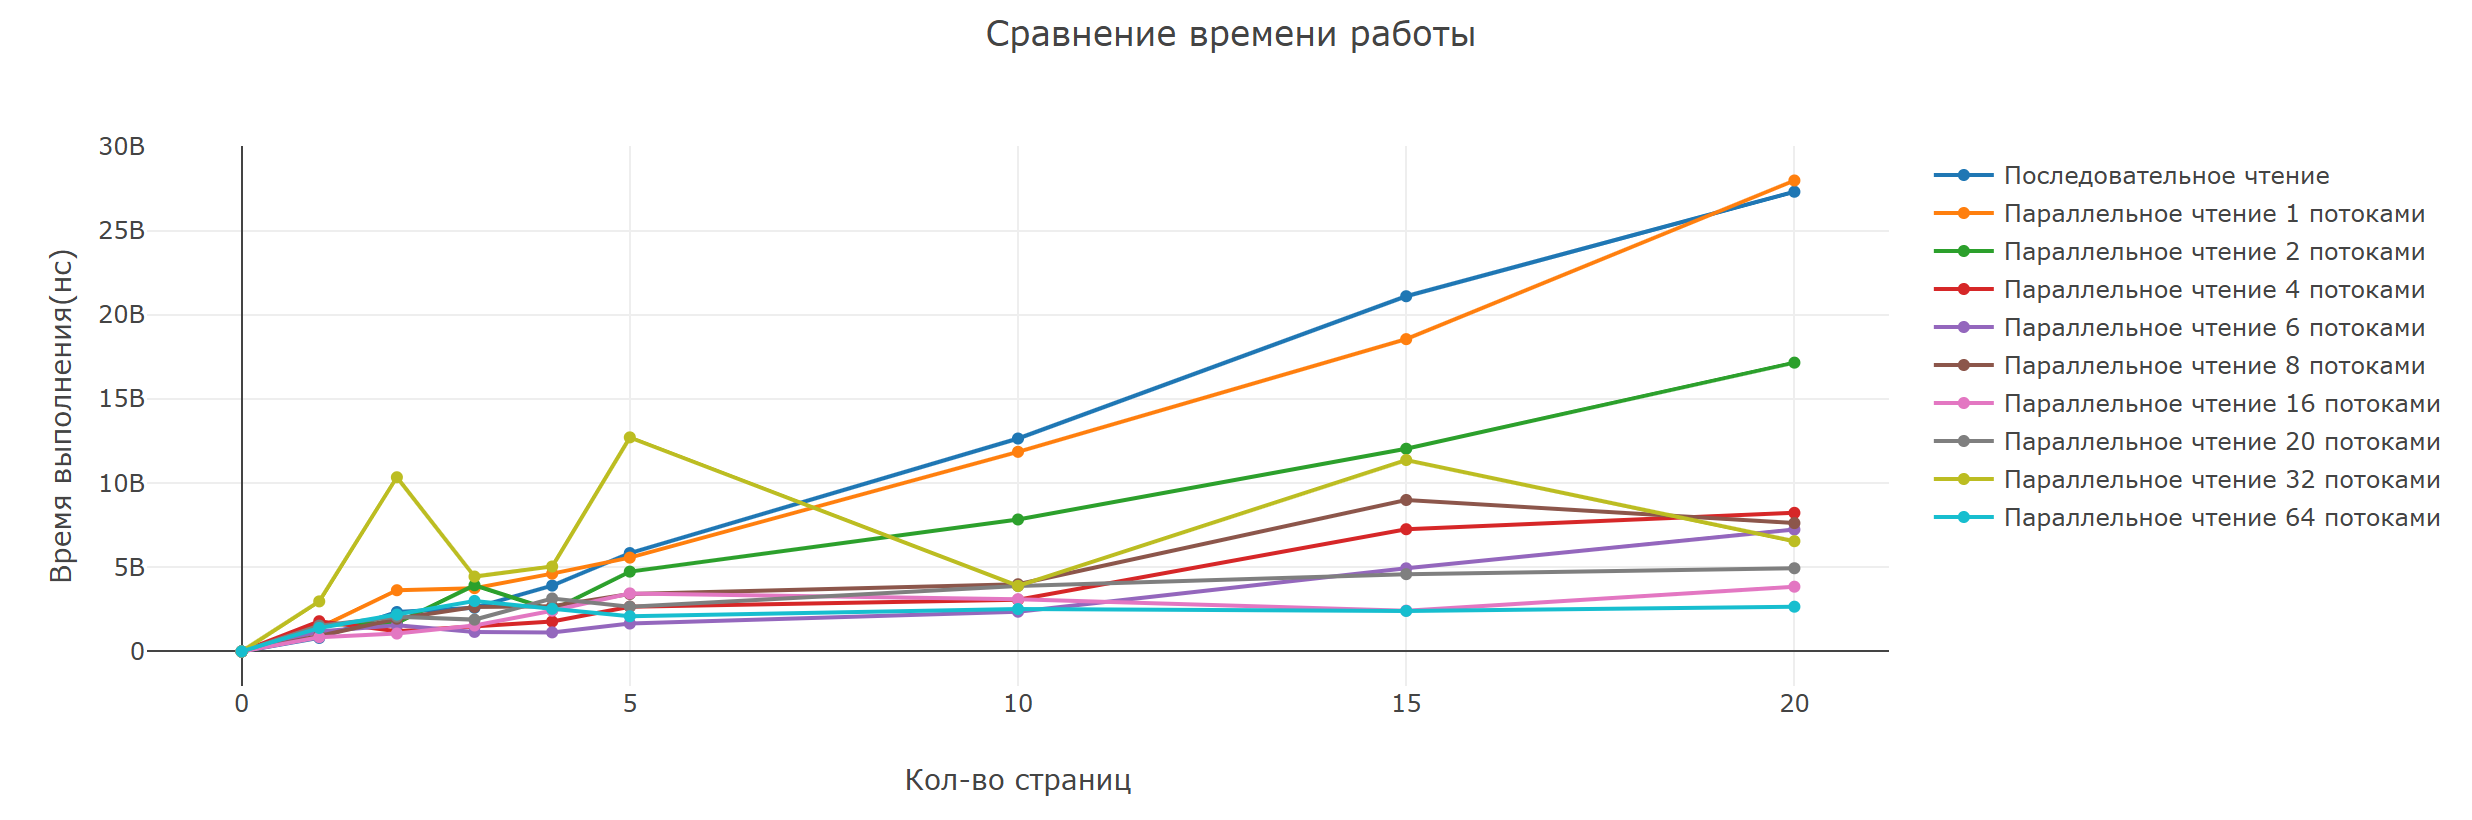
\includegraphics[width=0.8\textwidth]{images/plot.png}
	\caption{График зависимости времени выполнения от количества страниц}
	\label{fig:plot}
\end{figure}

\clearpage

Суммарное время загрузки всех страниц для каждого количества потоков представлено на таблице~\ref{tbl:mes}.

\begin{table}[h]
    \begin{center}
        \begin{threeparttable}
    \caption{Описание тестовых случаев}
    \captionsetup{justification=raggedright, singlelinecheck=false}
    \label{tbl:mes}
    \begin{tabular}{|r|r|}
        \hline
        \textbf{Количество потоков} & \textbf{Суммарное время работы(нс)} \\
        \hline
        0 & 76,607,837,500 \\
        \hline
        1 & 77,447,453,100 \\
        \hline
        2 & 51,466,208,900 \\
        \hline
        4 & 27,502,495,300 \\
        \hline
        6 & 21,266,895,200 \\
        \hline
        8 & 32,258,432,800 \\
        \hline
        16 & 18,734,472,100 \\
        \hline
        20 & 24,755,386,900 \\
        \hline
        32 & 57,397,960,200 \\
        \hline
        64 & 18,826,336,700 \\
        \hline
    \end{tabular}
    \end{threeparttable}
    \end{center}
\end{table}

В результате исследования было получено, что при использовании 16 потоков мы достигаем увеличение скорости в 3.2 раза относительно последовательной обработки. Также использование 16 потоков наиболее быстрое относительно других разбиений на потоки на процессоре с 12 ядрами и с 20 потоками, т.~к. мы используем не все доступные ресурсы, что позволяет избежать перегрузки системы и снижает накладные расходы на управление потоками.

\clearpage